\documentclass[12pt,titlepage]{report}

\usepackage{float}
\usepackage[T1]{fontenc}
\usepackage[utf8]{inputenc}
\usepackage{amsmath}
\usepackage{amssymb}
\usepackage[top=1.5cm, bottom=1.5cm, left=1.5cm, right=1.5cm]{geometry}
\usepackage{graphicx}
\usepackage{mathtools}
\usepackage[dvipsnames]{xcolor}
\usepackage{float}
\usepackage{multicol}
\usepackage{booktabs}
\usepackage{caption}
\usepackage{lipsum}
\usepackage{ragged2e}
\usepackage{hyperref}
\usepackage{enumitem}
\usepackage{eurosym}
\usepackage{indentfirst}
\usepackage{minted}
\usepackage{titlesec}
\usepackage{pifont}
\usepackage{url}
\usepackage{epsf}
\usepackage{algorithm}
\usepackage{algpseudocode}

\begin{document}

\begin{titlepage}
\newcommand{\HRule}{\rule{\linewidth}{0.5mm}}
\center
\textsc{\LARGE
CS203B: Mathematics For Computer Science-III
} \\[1cm]
\includegraphics[scale=0.18]{iitk.png} \\[1cm]
\HRule \\[0.4cm]
{ \huge \bfseries Assignment 2 \\[0.15cm] }
\HRule \\[2.5cm]
{\centering
\Large Aditya Tanwar\\[0.5cm]
\Large 200057}

\null\vspace{2cm}
\Large April 18, 2022 \\ [1cm]

\end{titlepage}

\newpage

\definecolor{boxgreen}{RGB}{221, 252, 189}
\newcommand{\ans}[1]{\colorbox{boxgreen}{\color{ForestGreen} #1}}
\newcommand{\loclink}[2]{\hyperlink{#1}{\color{NavyBlue} #2}}
\newcommand{\comment}[1]{&\pushright{\color{Gray} #1}}
\renewcommand{\o}[1]{$\mathcal{O}(#1)$}


\newpage

\section*{\hypertarget{q1}{Q1. Endsem Allocation}}

You are allocated as the Tutor of CS203, with $n$ students. Rajat has created 2 sets of Endsem papers to decrease cheating. He has asked you to help decide which paper should be given to whom. You scraped through the data on Hello, and found out who have been project partners in previous courses, as they will be friends now. Thus, you have found out $m$ friendship connections among the students. You reported this to Rajat, and he said he is fine with any allocation that disrupts atleast half of the
friendship connections. A friendship connection is disrupted if the students get different sets of papers.
\begin{enumerate}[label=(\alph*)]
    \item You are really busy, and just randomly allocated each student to set 1 or set 2. Show that the expected value of disrupted friendship connections is $\frac{m}{2}$.
    \item[\underline{\textit{Solution:}}] Let the set of friendship connections be denoted by $M$, and an element of $M$ be denoted by $f$. By slight abuse of notation, we write $f=0$ to mean that the friendship connection was not disrupted and $f=1$ to mean that it was disrupted. Similarly, for a student $s_0$, we write $s_0=1$ to mean that the student $s_0$ was assigned the set 1, and $s_0=2$ to mean that set 2 was assigned. We also write $f(s_1, s_2)$ to mean the value of $f$ corresponding to the assignment that $s_1$ and $s_2$ have ($s_1,s_2$ are the two students in the friendship).\\
    Then, for any friendship connection $f_0\in M$, consisting of two students, say $s_1$ and $s_2$, there are four possible assignments- 
    $$\langle 1,\,1 \rangle,\ \langle 1,\,2 \rangle,\ \langle 2,\,1 \rangle,\ \langle 2,\,2 \rangle$$
    Out of these 4 equi-probable cases, only 2 are of interest to us, namely $\langle 1, 2\rangle$ and $\langle 2, 1 \rangle$, since they disrupt $f_0$. Therefore, two of the assignments result in $f_0=1$ and two result in $f_0=1$.
    Equipped with this knowledge, we calculate the expected value of $f_0$,
    \begin{align*}
        E[f_0]=0\cdot \frac{1}{4}+1\cdot \frac{1}{4}+1\cdot \frac{1}{4}+0\cdot \frac{1}{4} =\boxed{\frac{1}{2}}
    \end{align*}
    Let $l$ denote the number of friendship connections disrupted in a particular assignment, then we can write,
    \begin{align*}
        l&=\sum_{f\in M} f(s_1, s_2) \comment{\textit{where $s_1$ and $s_2$ are the students in $f$}}
    \end{align*}
    Thus,
    \begin{align*}
        E[l] &= E\left[\sum_{f\in M} f(s_1, s_2)\right] \\
        &= \sum_{f\in M} E[f(s_1,s_2)] \comment{\textit{ By linearity of expectation}} \\
        &= \sum_{f\in M} \frac{1}{2} = \frac{1}{2}\cdot m \comment{\text{$\because\ |M|=m$}} \\
        &= \ans{$\dfrac{m}{2}$}
    \end{align*}
      
    \item Getting expected value is not enough, you need to find a proper allocation. But you cannot go over all the $2^n$ allocations as $n\approx 150$. Using the construction for pairwise independence given in class, show that you can find an allocation with at least half of the friendship connections disrupted in poly($n$)-time.
    \item[\underline{\textit{Solution:}}] We first re-formulate the problem into a graph problem, where each student is replaced a vertex, and the friendship connections are replaced by edges between vertices. We shall provide a greedy algorithm which runs in \o{n^3} time which can be decreased to \o{n^2} runtime with some minor optimizations (and usage of appropriate data structures).\\
    The pseudo-code of the algorithm follows after the notations.
    \begin{itemize}
        \item $\delta_S(v)\coloneqq$ The number of edges with the vertex $v$ at one end, and a vertex from the set $S$ on the other end.
        \item $V\coloneqq$ Vertex Set, $E\coloneqq$ Edge Set, $S_1\coloneqq$ Set of students that get the first paper set, similarly for $S_2$.
        \item \textit{Disruptions:} Function that takes two sets as input and returns the number of edges ``disrupted'' by the assignment (from the two sets). Essentially, counts the number of edges having one end in the first set and the other end in the second set.\\
        ``Disrupted'' follows the same definition as in the question.
    \end{itemize}
    
    \begin{algorithm}
    \caption*{\textbf{Algorithm}}
    \begin{algorithmic}
    \State $S_1 \gets \varnothing,\,S_2\gets\varnothing$
    \For{$v\in V$}
    \State Calculate $\delta_V(v)$
    \EndFor
    \State Sort $V$ in descending order of $\delta_V(v)$
    \For{$v\in V$}
    \If{$\delta_{S_1}(v)>\delta_{S_2}(v)$}
    \State $S_2\gets S_2\cup \{v\}$
    \Else
    \State $S_1\gets S_1\cup\{v\}$
    \EndIf
    \If{\textit{Disruptions($S_1,S_2$)}$>{|E|}/{2}$}
    \State $S_1\gets V\backslash S_2$
    \State \textbf{break}
    \EndIf
    \EndFor
    \State \textbf{return} $S_1,\,S_2$
    \end{algorithmic}
    \end{algorithm}
\end{enumerate}
    Firstly, the \underline{proof of run-time}. There are majorly four steps involved in the algorithm, the run-time of each is elaborated-
    \begin{itemize}
        \item Calculation of $\delta_V(v)$: This can be calculated in \o{n} per vertex with a representation like adjacency matrix or adjacency list. Thus, overall complexity is \o{n^2}.
        \item Sorting: Can be sorted in \o{n\log{n}}. 
        \item Computing $\delta_{S_1}(v)$ and $delta_{S_2}(v)$: Similar to $\delta_V{v}$, it can be calculated in \o{n} per vertex, thus the cumulative run-time (summed over the for loop) is \o{n^2} or \o{n^2}.
        \item Disruptions: Can be calculated naively in \o{|S_1||S_2|}=\o{n^2} per iteration, cumulative run-time thus being \o{n^3}.
    \end{itemize}
    Summarising, the run-time is \o{n^3}. This can be improved to \o{n^2}, subject to the fact that \textit{(i)} we can find what set a vertex belongs to, in \o{1} \textit{(can be done by storing an array)} and \textit{(ii)} instead of recomputing the number of disruptions for each iteration, we maintain a variable for it and update it in \o{n}. The run-time of loop would thus be brought down to \boxed{\mathcal{O}(n^2)}.\\
    
    Now, \underline{proof of correctness}. \\
    At the time of insertion of any vertex $v$, we consider only its ``active'' edges (edges corresponding to vertices from $S_1$ or $S_2$). The rest of the edges of $v$ are considered later at the time of insertion of some other vertex. It is a key observation to make that each edge is considered at most once.
    
    Further, at the time of insertion of any vertex, at least half of the ``active'' edges are disrupted. Since at each individual disruption, at least half of the edges are disrupted, at the time of termination of the algorithm, either \textit{(i)} each edge will have been considered at least once, thus resulting in half of the edges having been disrupted, or \textit{(ii)} it will have terminated due to the \textit{break} statement, in which case ofcourse, at least half the edges have been disrupted.\\ \\
    
    Thus, concluding the proof of \ans{correctness} of the algorithm, as well as proving that it runs in \ans{poly(\textit{n})-time}.
\newpage


\section*{\hypertarget{q2}{Q2. Estimating the number of tickets}}

You are given a bag full of $N$ tickets numbered $1, \dots , N$ ($N$ is unknown to you). You can take out tickets one at a time, note their label, and put them back in the bag. Your task is to estimate $N$. We will do this in the same way as we estimated $\pi$ in lecture:

\begin{enumerate}[label=(\alph*)]
    \hypertarget{q2a}{\item} Assume you drew out $k$ tickets. What will be the expected value of the mean of these tickets? Calculate $N$ in terms of this mean, call this $\widetilde{N}$.
    \item[\underline{\textit{Solution:}}] Let $X_i$ be the random variable that takes the value of the $i^{th}$ ticket drawn, $S_k\coloneqq \sum_{i=1}^{i=k} X_i$ denote the sum, and $M_k\coloneqq\frac{S_k}{k}$ denote the mean. \\
    We first find the expected value of $X_i$. $X_i$ can take any value from the integers between 1 and $N$ (both inclusive) with equal probability, $p=\frac{1}{N}$,
    \begin{align*}
        E[X_i] &= \sum_{j=1}^{j=N} j\cdot p = \sum_{j=1}^{j=N} j \cdot \frac{1}{N}\\
        &= \frac{1}{N} \sum_{j=1}^{j=k} j = \frac{1}{N} \cdot \frac{N(N+1)}{2} \\
        &= \boxed{\frac{N+1}{2}}
    \end{align*}
    Since, the set $\{X_i\}$ represents a set of \href{https://en.wikipedia.org/wiki/Independent_and_identically_distributed_random_variables}{\color{Cerulean} \textit{I.I.D. RV's}}, each $X_i$ has the same expected value. Thus, to calculate the mean, we write,
    \begin{align*}
        E[M_k] &= E\left[\frac{1}{k}\sum_{i=1}^{i=k} X_i\right] \\
        &= \sum_{i=1}^{i=k} \frac{1}{k}\cdot E[X_i] \comment{\color{Gray} \textit{From linearity of expectation}} \\
        &= \frac{1}{k} \sum_{i=1}^{i=k} \frac{N+1}{2} = \frac{1}{k} \frac{k(N+1)}{2}\\
        &= \ans{$\dfrac{N+1}{2}$} \comment{\textit{The expected value of mean}}
    \end{align*}
    Let the value of the mean be $M_k$. Then by the above result, we write,
    \begin{align*}
        M_k=\frac{\widetilde{N}+1}{2} \Rightarrow \ans{$\widetilde{N}=2M_k-1$}
    \end{align*}
    
    \item Chernoff bound can be extended to work on the case when the Random Variables take values other than ${0, 1}$. This is known as Hoeffding’s inequality. Use it to find a lower bound on the probability that the error in $N$, using the above calculation, will be less than $\delta N\,(\delta < \frac{1}{2})$. (in terms of $N,\, \delta,\, k$)
    \item[\underline{\textit{Solution:}}] We first write the expression for \href{https://en.wikipedia.org/wiki/Hoeffding\%27s_inequality#Statement}{\textit{\color{Cerulean} Hoeffding's Inequality}} and manipulate it to suit our cause,
    \begin{align*}
        P(|S_k-E[S_k]|\geq t)&\leq 2\exp{\left(-\frac{2t^2}{\sum_{i=1}^{i=k} (b_i-a_i)^2}\right)}\\
    \end{align*}
    We observe that since $S_k=k\cdot M_k$, we have, $E[S_k]=k\cdot E[M_k]=k\cdot\frac{N+1}{2}$ and since $X_i$ are \href{https://en.wikipedia.org/wiki/Independent_and_identically_distributed_random_variables}{\color{Cerulean} \textit{I.I.D. RV's}}, with $1\leq X_i\leq N\,\forall i\in [k]$, we get $a_i=1$ and $b_i=k\, \forall i\in[k]$. Using $S_k=k\cdot M_k=k\cdot \frac{\widetilde{N}+1}{2}$ So,
    \begin{align*}
        P\left(|k\cdot \frac{\widetilde{N}+1}{2}-k\cdot \frac{N+1}{2}|\geq t\right)&\leq 2\exp{\left(-\frac{2t^2}{\sum_{i=1}^{i=k} (N-1)^2}\right)}\\
        P\left(\frac{k}{2}\cdot|\widetilde{N}-N|\geq t\right)&\leq 2\exp{\left(-\frac{2t^2}{k\cdot(N-1)^2}\right)}\\
        P\left(|\widetilde{N}-N|\geq \frac{2t}{k}\right)&\leq 2\exp{\left(-\frac{2t^2}{k\cdot(N-1)^2}\right)}\\
    \end{align*}
    We shall find the probability $P(|\widetilde{N}-N|\geq \delta N)$ and then complement it to compute the desired probability. Thus, we require,
    \begin{align*}
        |\widetilde{N}-N|&\geq \delta N \qquad |\widetilde{N}-N|\geq \frac{2t}{k}\\
        &\Rightarrow \delta N=\frac{2t}{k}\\
        &\Rightarrow \boxed{t=\frac{k\delta N}{2}}
    \end{align*}
    Putting this result in the inequality, we get,
    \begin{align*}
        P(|\widetilde{N}-N|\geq \delta N) &\leq 2\exp{\left(-\frac{2(k\delta N/2)^2}{k\cdot(N-1)^2}\right)}\\
        &\leq \boxed{2\rm{e}^{-k\delta^2 N^2/2(N-1)^2}=2\,\exp{\left(-\frac{k\delta^2}{2}\frac{ N^2}{(N-1)^2}\right)}}
    \end{align*}
    Since the events $|\widetilde{N}-N|\geq{\delta N}$ and $|\widetilde{N}-N|<\delta N$ are complementary, we can write,
    \begin{align*}
        P(|\widetilde{N}-N|<\delta N) &= 1-P(|\widetilde{N}-N|\geq{\delta N})\\
        &\geq \ans{$1-2\,\exp{\left(-\dfrac{k\delta^2}{2}\left(\dfrac{N}{N-1}\right)^2\right)}$}
    \end{align*}
    
    \item Assume $k, N$ are odd. In calculation of \loclink{q2a}{part $(a)$}, instead of using the value of mean, we use the median of the labels of tickets drawn. Prove a lower bound of $1-2e^{-\frac{k(1+2\delta)^2}{2(3-2\delta)}}$ on the probability that the error in $N$ using the median will be less than $\delta N\,(\delta < \frac{1}{2})$. (in terms of $N,\, \delta,\, k$)
    \item[\underline{\textit{Solution:}}] Let $M_e$ denote the median of the tickets drawn. We claim that $E[M_e]=(N+1)/2$ (since $k$ is odd). \\
    A short proof from symmetry foolows. For any $1\leq i\leq N$, $$P(M_e=i)=P(M_e=N+1-i)$$ This follows from the fact that for any sequence of ticket draws, say $D_i$, having median $(i)$, a corresponding, equiprobable event $D_{N+1-i}$ exists which has median $(N+1-i)$. $D_{N+1-i}$ can be constructed easily from $D_i$ by simply replacing each entry $x\in D_i$ by $(N+1-x)$ in $D_{N+1-i}$. Thus, the number of draws having median $i$ is equal to the number of draws having median $N+1-i$. Now, to calculate the expected value of median, we write,
    \begin{align*}
        E[M_e] &= \sum_{i=1}^{i=N} i\cdot P(M_e=i) \\
        \Rightarrow 2\,E[M_e] &= \sum_{i=1}^{i=N} i\cdot P(M_e=i) + \sum_{j=1}^{j=N} j\cdot P(M_e=j) \\
        &= \sum_{i=1}^{i=N} i\cdot P(M_e=i) + \sum_{i=1}^{i=N} (N+1-i)\cdot P(M_e=N+1-i) \comment{\textit{Letting $j=N+1-i$}} \\
        &= \sum_{i=1}^{i=N} (i+N+1-i)\cdot P(M_e=i) \comment{\because P(i)=P(N+1-i)} \\
        &= (N+1)\cdot \sum_{i=1}^{i=N} P(M_e=i) = (N+1) \\
        &\Rightarrow \boxed{E[M_e]=\frac{N+1}{2}}
    \end{align*}
    
    \hypertarget{q2c}{\item} Start with a random hidden value of $N$ in range $10^4-10^6$. Write a function that gives $k$ values from $[N]$ when queried with equal probability. Use these values to calculate $\widetilde{N}$ as in \loclink{q2a}{part $(a)$} and \loclink{q2c}{part $(c)$}, and plot them with respect to increasing $k \leq 1000$. Repeat this estimation for a total of 3 different $N$, and put the plots in the main answer file. Submit the code you used to generate these plots, along with a \texttt{readme} on how to execute the code, zipped together with the main answer file into a single \texttt{.zip} file.
    {\begin{figure}[!ht]
        \centering
        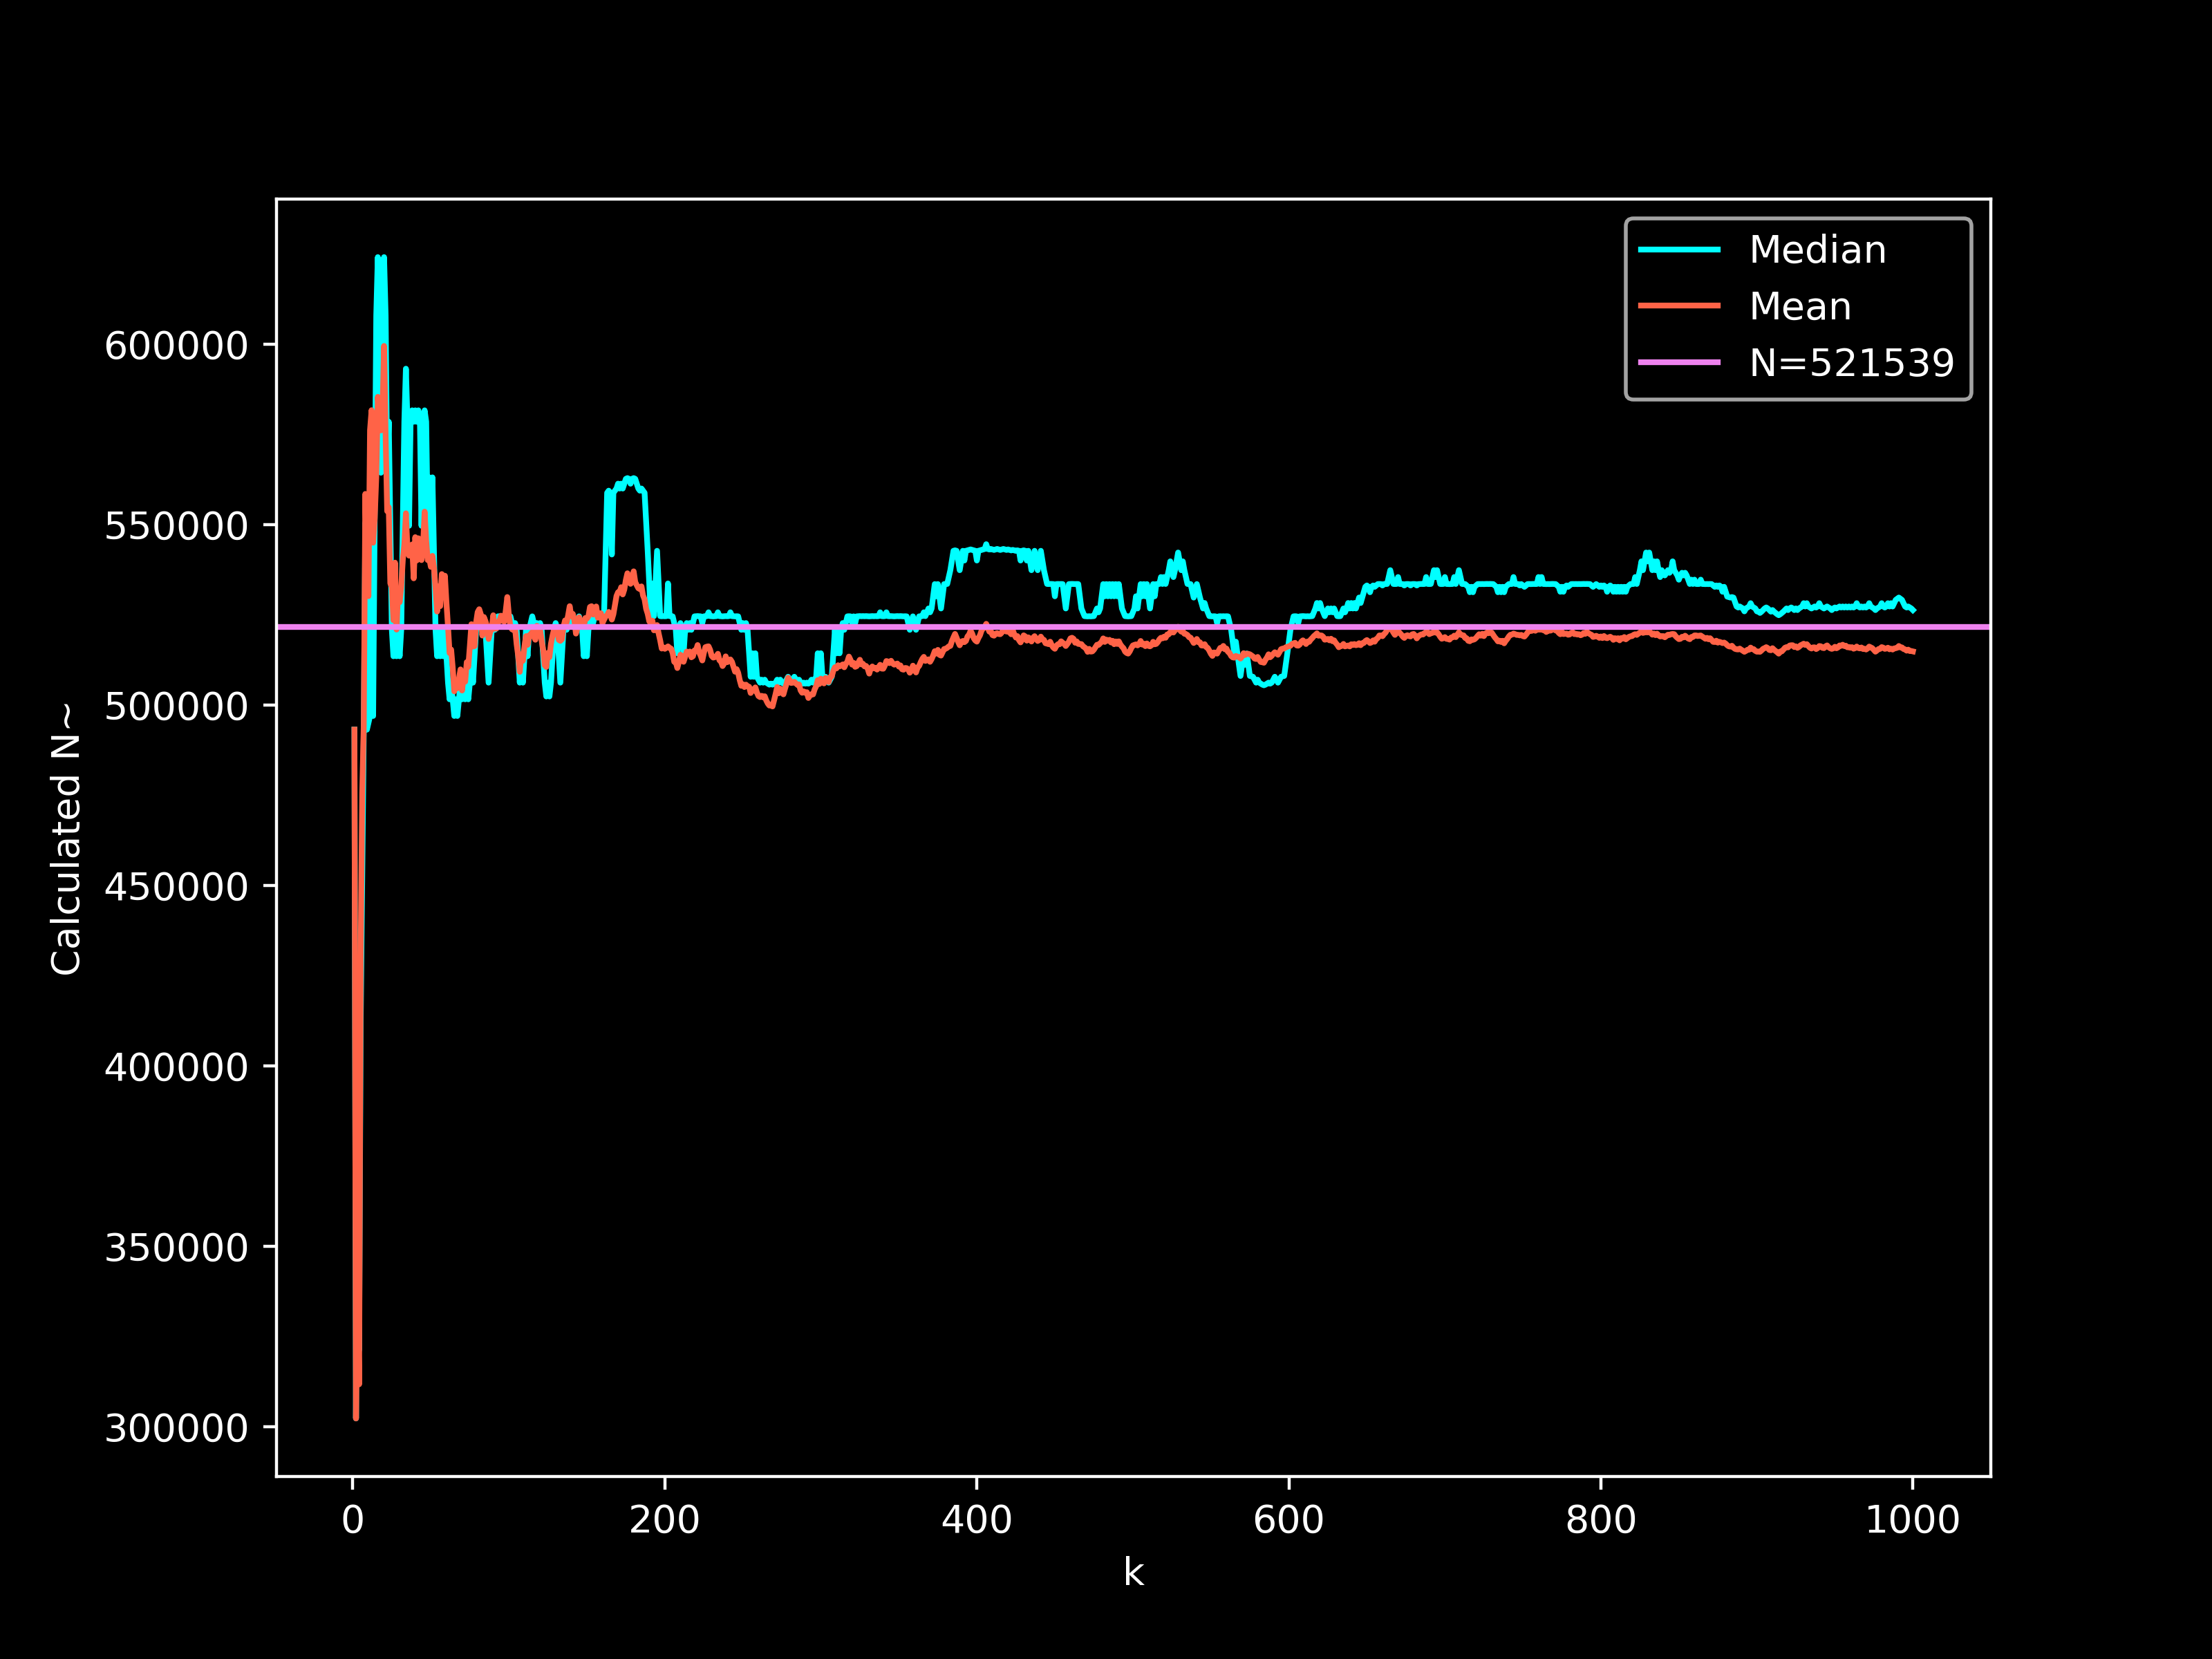
\includegraphics[scale=0.7]{200057_n_521539.png}
    \end{figure}}
    {\begin{figure}[!ht]
        \centering
        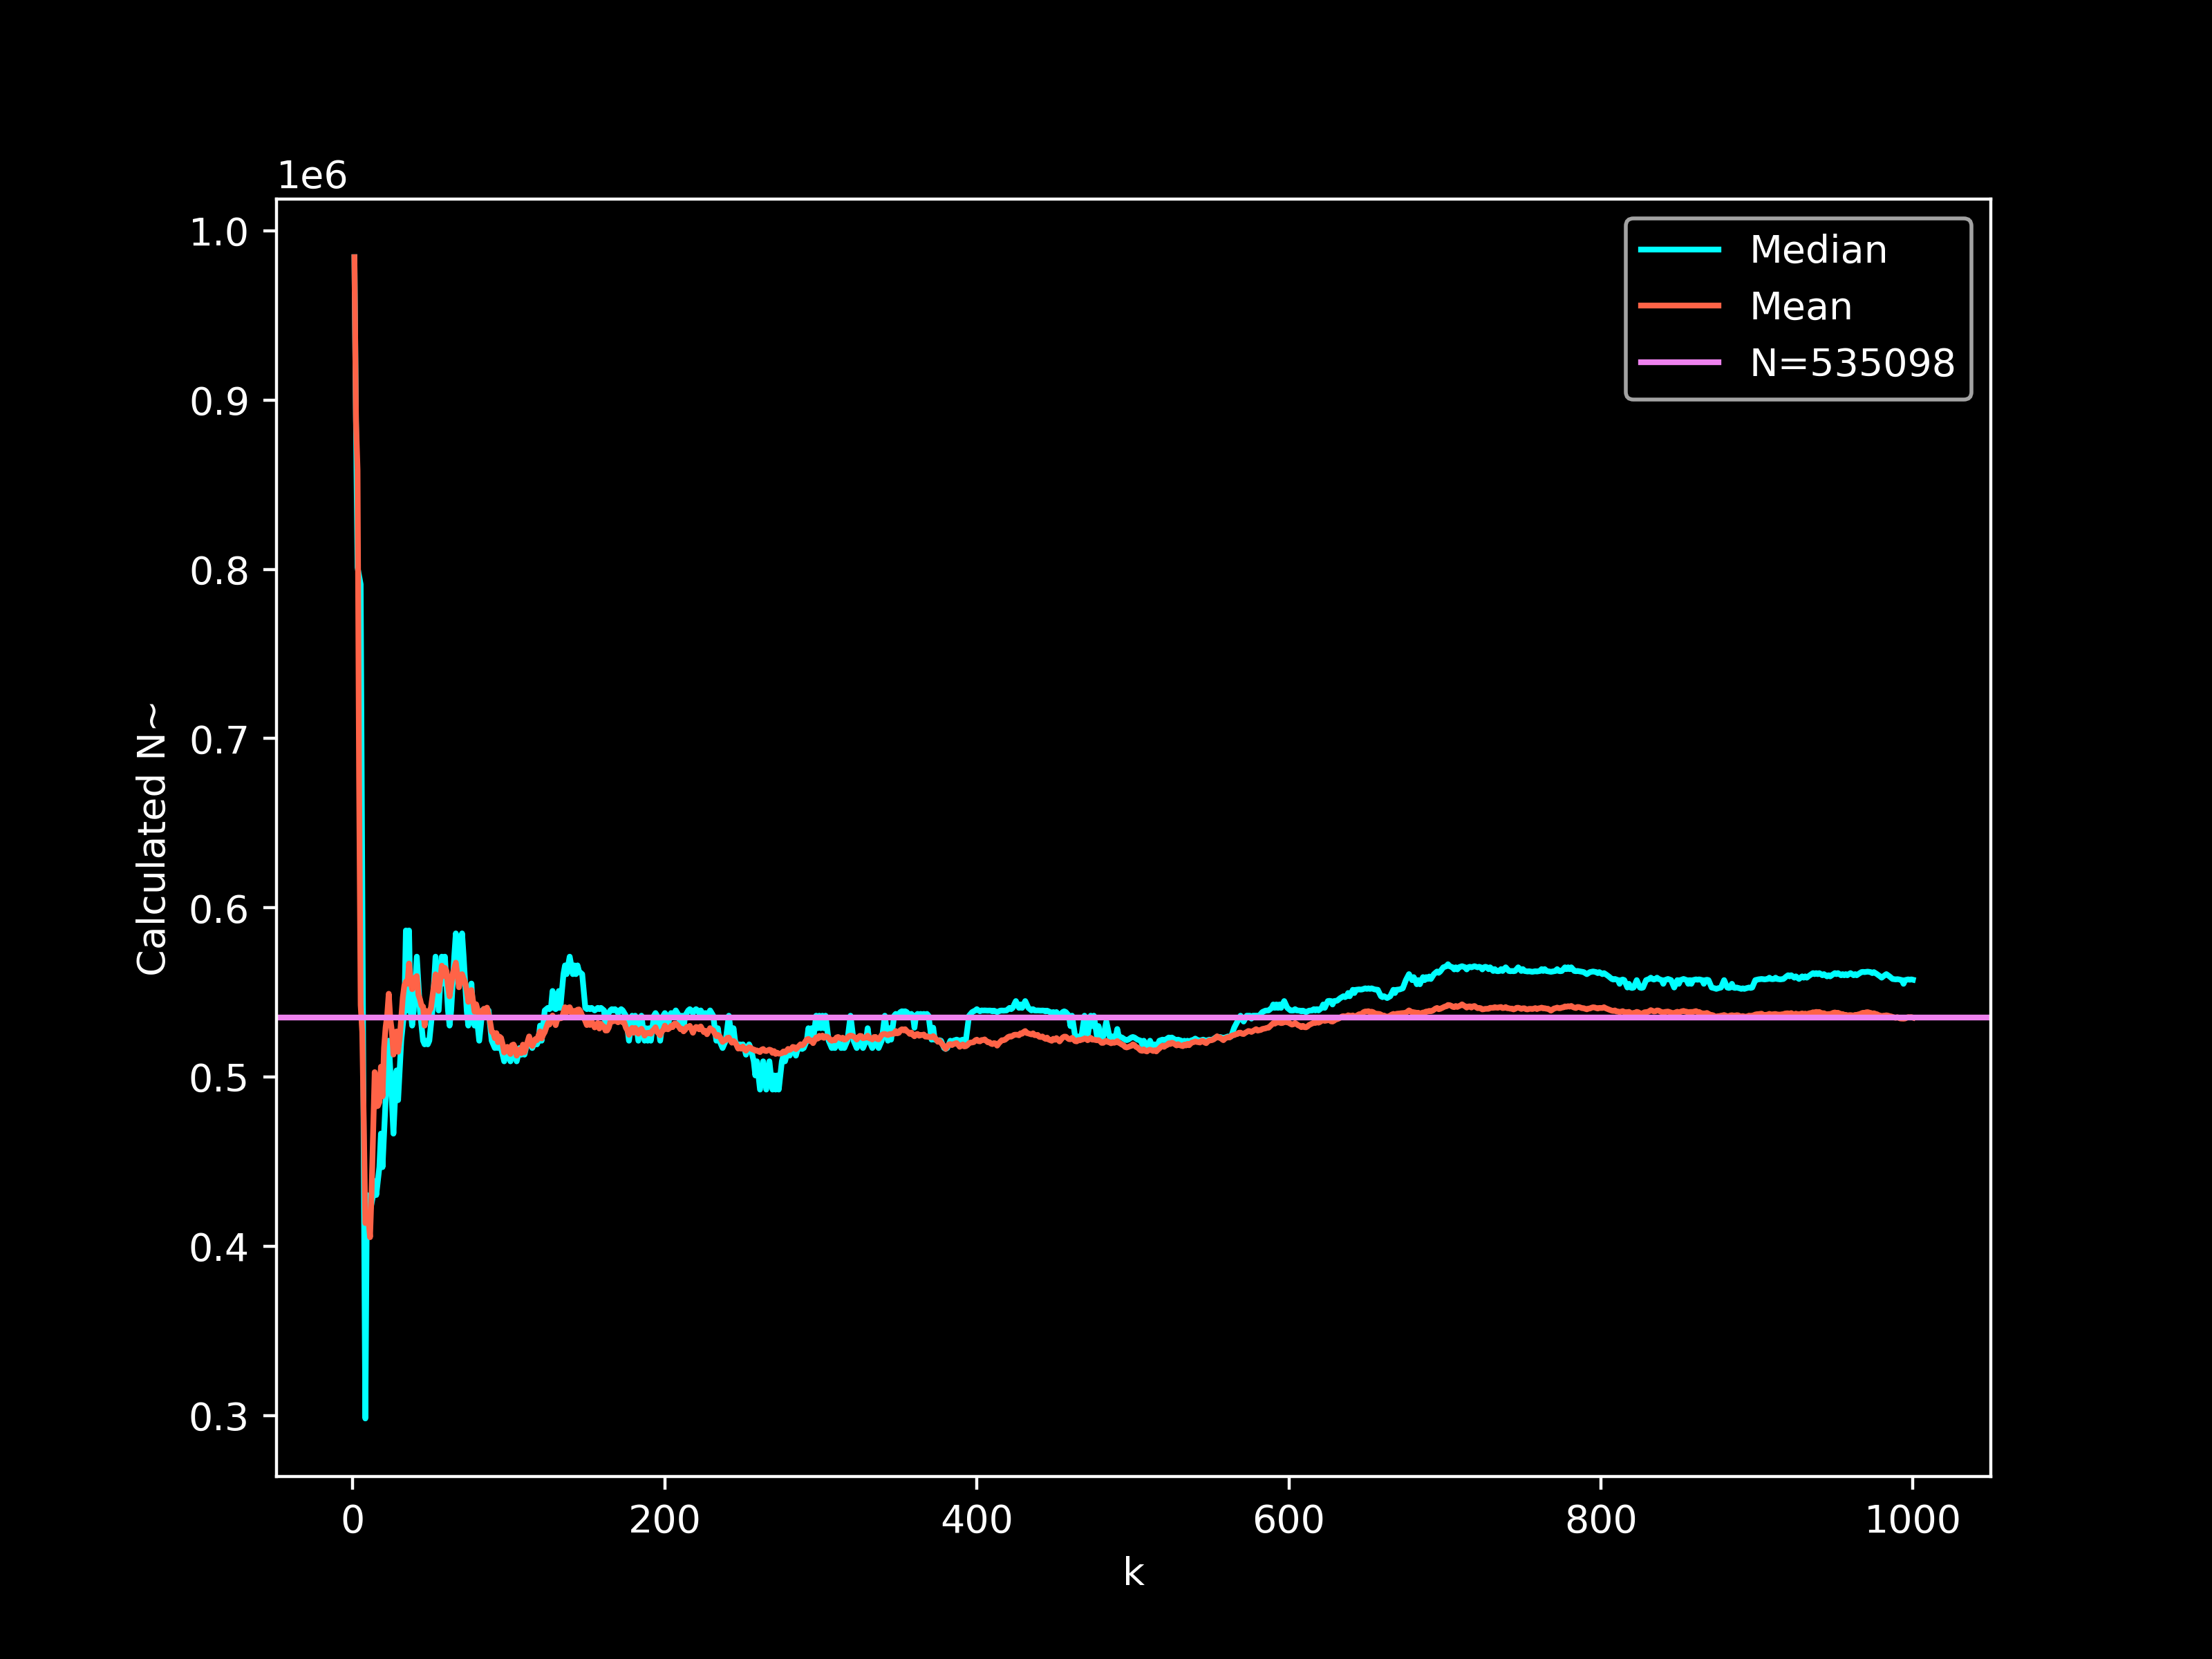
\includegraphics[scale=0.7]{200057_n_535098.png}
    \end{figure}}
    {\begin{figure}[!ht]
        \centering
        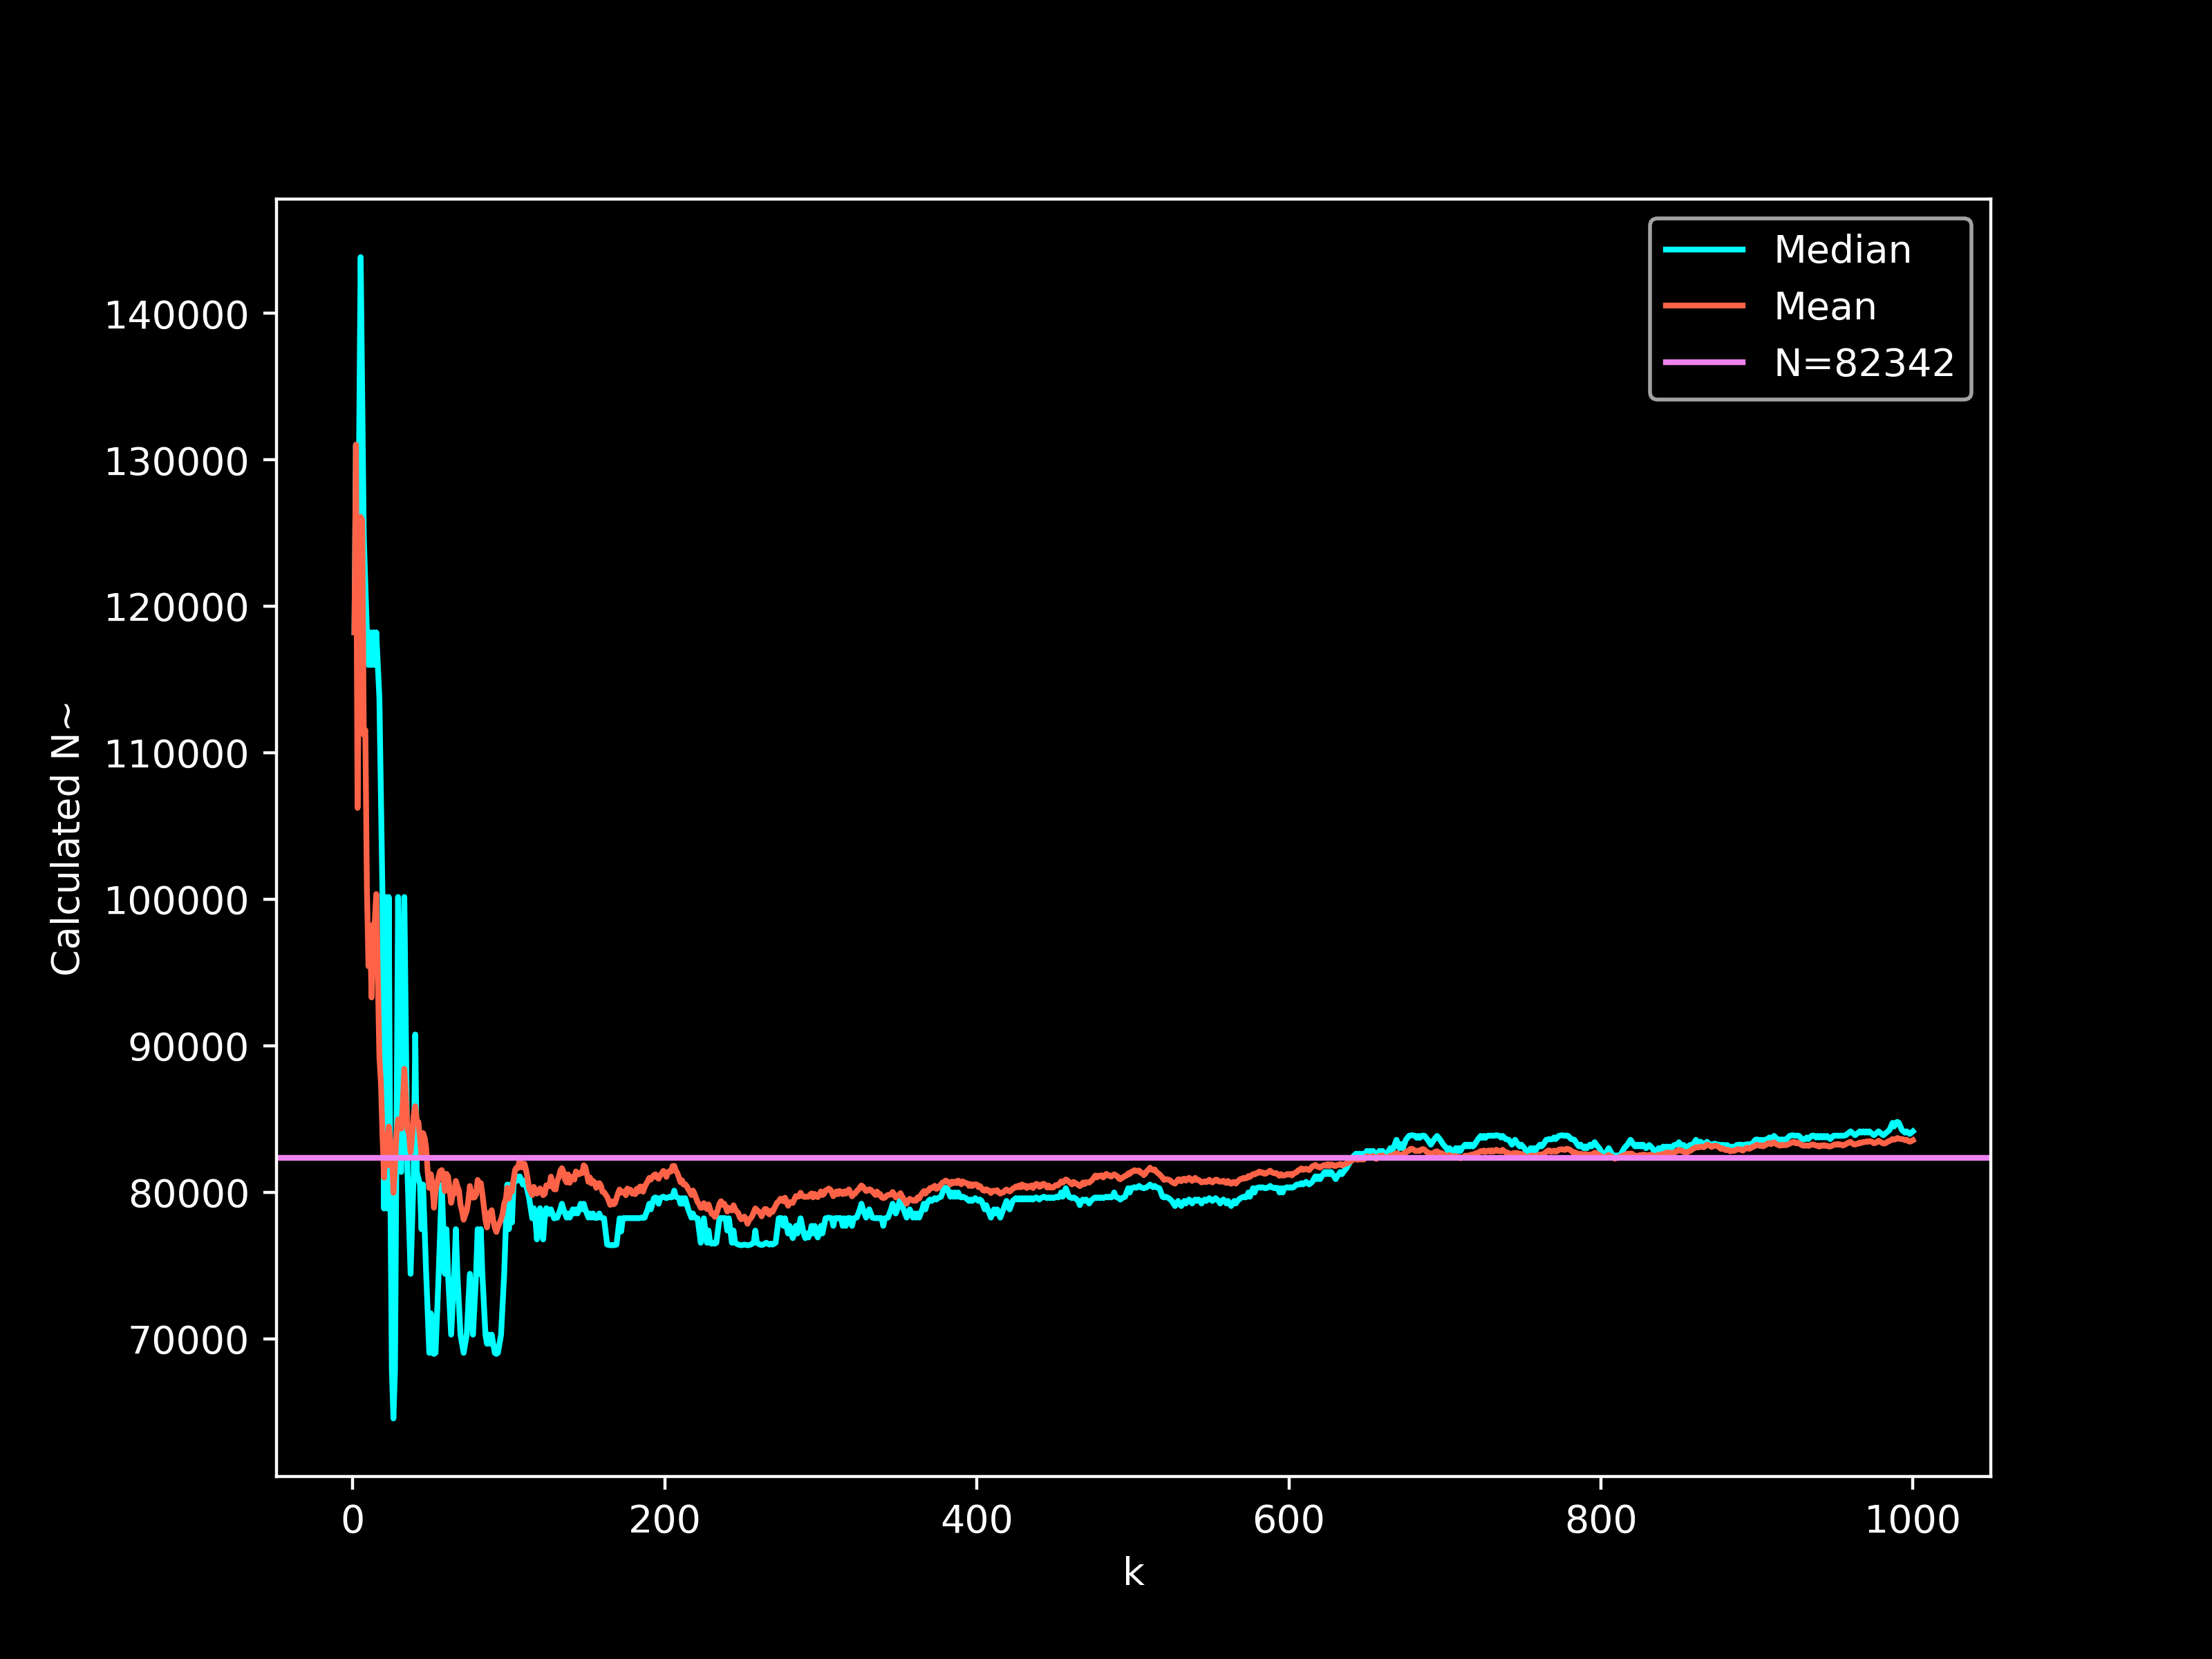
\includegraphics[scale=0.7]{200057_n_82342.png}
    \end{figure}}
    \item[\textit{Comments:}] 
    The mean and median have not been rounded off, they have instead been plotted as is.
    The plot with the median seems to have a higher variance than the plot with the mean, but the variance of both the plots decreases with increasing $k$ and the plots come closer to the actual value of $N$ as a general rule.
\end{enumerate}

\clearpage

\section*{\hypertarget{q3}{Q3. Markov Chain}}

Consider a homogeneous regular Markov chain with state space $S$ of size $|S|$, and transition matrix $M$. Suppose that $M$ is symmetric and entry-wise positive.
\begin{enumerate}[label=(\alph*)]
    \hypertarget{q3a}{\item} Show that all the eigenvalues of $M$ are bounded by 1 and that the uniform distribution is the unique stationary probability distribution for $M$.
    \item[\underline{\textit{Solution:}}] Towards contradiction, assume $\exists\, \lambda_0$ an eigenvalue of the Markov matrix $M$ such that $|\lambda_0|>1$. Let $u_0\neq \mathbf{0}$ be any eigenvector corresponding to $\lambda_0$, then we can write-
    \begin{align*}
        u_0M=\lambda_0u_0 \Rightarrow u_0 &= u_0\frac{M}{\lambda_0} \\
        \Rightarrow u_0 &= u_0\left(\frac{M}{\lambda_0}\right)^l \comment{\textit{By repeated substitution} \qquad  (l\in\mathbb{N}}) \\
        &= u_0\lim_{l\rightarrow\infty} \left(\frac{M}{\lambda_0}\right)^l \\
        &= u_0\mathbf{O} \comment{0\leq(M^n)_{i,j}\leq1\,\forall\,i,j\quad \&\quad |\lambda_0|>1} \\
        u_0&= \mathbf{0}
    \end{align*}
    Which is a contradiction since a non-zero eigenvector must exist corresponding to each eigenvalue, hence no eigenvalue of a Markov Matrix can exceed 1. The eigenvalues of $M$ are thus \ans{\textit{bounded by 1}}\\ \\
    \underline{Note:} $0\leq(M^n)_{i,j}\leq1$ since $(M^n)_{i,j}$ is the probability of reaching $j$ after $n$ steps having initially started at $i$. Proof is by induction on the number of steps. The explanation for $n=1,2$ has already been given in the notes. We assume it to hold for $n=k$. Now, $$P(X_{k+1}=j| X_0=i)=\sum_{u\in S}\,P(X_{k+1}=j|X_k=u)\cdot P(X_k=u|X_0=i)$$
    by simply enumerating all the possibilities.\\
    By homogeneous nature of $M$, we have $P(X_{k+1}=j|X_k=u)=P(X_1=j|X_0=u)=M_{u,j}$. \\
    And by the Induction Hypothesis, we have, $P(X_k=u|X_0=i)=(M^k)_{i,u}$. \\
    Thus, we have,
    $$P(X_{k+1}=j| X_0=i)=\sum_{u\in S} M_{u,j}\cdot(M^k)_{i,u}\Rightarrow P(X_{k+1}=j| X_0=i)=(M^{k+1})_{i,j}$$
    by properties of Matrix multiplication. This completes our proof.\\
    The stationary probability distribution for $M$, is a (column) vector $u$ such that $u^T=u^TM$. Let $u_0=\mathbf{1}/|S|$ be the uniform distribution. We first show that it is a stationary probability distribution of $M$,
    {\allowdisplaybreaks
    \begin{align*}
        (u_0^TM)_i &= \sum_{j\in[|S|]} u_j\cdot M_{j,i} \\
        &= \frac{1}{|S|} \sum_{j\in[|S|]} M_{j,i} \comment{u_k=\frac{1}{|S|}\,\forall\, k\in[|S|]} \\
        &= \frac{1}{|S|} \sum_{j\in[|S|]} M^T_{i,j} \\
        &= \frac{1}{|S|} \sum_{j\in[|S|]} M_{i,j} \comment{\because\, M \textit{ is symmetric}}\\
        &\boxed{(u_0^TM)_i = \frac{1}{|S|}} \comment{\textit{Sum of rows of $M$ (Markov Matrix) is 1}}
    \end{align*}}
    As each entry in the vector $(u_0^TM)$ is $\frac{1}{|S|}$, it is the uniform distribution, or in other words, $u_0^TM=u_0^T$. So, we know that $u_0$ is a \boxed{\text{stationary distribution}} of $M$. \\ \\
    Clearly, $\lambda_0=1$ is an eigenvalue of $M$, since $u_0^T=u^T_0M$. As all eigenvalues of $M$ are bounded by 1, $\lambda_0=1$, and $M$ is entry-wise positive, by \href{https://en.wikipedia.org/wiki/Perron\%E2\%80\%93Frobenius_theorem}{\color{Cerulean}\textit{Perron--Frobenius Theorem}}, we have $\mu_M(\lambda_0)=1$. Since $1\leq\gamma_M(\lambda_0)\leq\mu_M(\lambda_0)$, $\gamma_M(\lambda_0)$ is forced to be 1, thus implying the \boxed{\text{uniqueness}} of $u_0$. \\
    \textit{($\mu_M$ and $\gamma_M$ have been elaborated in the \loclink{app}{appendix})}\\ \\
    Combining these results, we get that $u_0=\mathbf{1}/{|S|}$ is the \ans{\textit{unique stationary distribution}} of $M$.
    
    \item Starting from the stationary distribution, express the probability of returning to the same state as the state at $t = 0$ after $n \in \mathbb{N}$ steps in terms of the eigenvalues of $M$. Compute the limit of the above probability as $n\rightarrow \infty$.
    We claim that if $\lambda$ is an eigenvalue of $A$ then $\lambda^n$ is an eigenvalue of $A^n$. The proof follows from the simple fact that $A=\lambda I\Rightarrow A^n = (\lambda I)^n = \lambda^n I^n=\lambda^n I$.\\
    \item[\underline{\textit{Solution:}}] Let $\Lambda_M$ be the multiset of all the eigenvalues of the Markov Matrix $M$. Essentially, we want to find
    $$\sum_{i\in[|S|]} P(X_n=i|X_0=i)\cdot P(X_0=i) = \sum_{i\in[|S|]} (M^n)_{i,i} \cdot\frac{1}{|S|}$$
    The first substitution has already been proved above in \loclink{q3a}{part (a)}, and the second substitution comes from starting from stationary distribution, i.e., the uniform distribution.
    
    \begin{align*}
        \sum_{i\in[|S|]} P(X_n=i|X_0=i)\cdot P(X_0=i) &= \frac{1}{|S|}\sum_{i\in[|S|]} (M^n)_{i,i} \\
        &= \frac{\text{Tr($M^n$)}}{|S|} \comment{\textit{Tr is short for Trace}} \\
        &= \ans{$\dfrac{\sum_{\lambda\in\Lambda_M}\lambda^n}{|S|}$}
    \end{align*}
    As $n\rightarrow\infty$, all terms corresponding to $|\lambda|<1$ will vanish and only the term corresponding to $\lambda_0=1$ will survive, thus, the probability will become \ans{$\dfrac{1}{|S|}$}.\\
    Another way to show this is by observing that $\lim_{n\rightarrow\infty} M^n=M_\infty=\mathbf{J}/|S|$. This follows from the fact that each column of $M_\infty$ is the same. Since $M$ is a symmetric matrix, all rows are also the same. Combining these two results, we obtain that $M_\infty=c\cdot \mathbf{J}$. As the sum of entries in a column of $M_\infty$ is 1, we obtain $c=1/|S|$. Thus, Tr($M_\infty$)$=\sum_{i\in[|S|]} 1/|S| = 1$, and hence the probability is $1/|S|$.
\end{enumerate}
    Feel free to assume the first part and finish the second part (if you can’t prove the first part).

\newpage

\section*{\hypertarget{q4}{Q4. DNF Counting}}
\vspace{-1cm}
\null\hfill \textit{(Optional)}\\
Given a DNF formula $F$ of $n$ variables, how can we estimate the number of satisfying assignments without considering all cases? A natural approach is to randomly sample $m$ assignments uniformly from the set of all possible assignments. Let $X$ be the number of satisfying assignments among the $m$ samples.
\begin{enumerate}[label=(\alph*)]
    \item Derive an unbiased estimate for the total number of satisfying assignments in terms of $X, m, n$.
    \item[\underline{\textit{Solution:}}] We simply scale the solutions we saw to the total number of cases possible. Let the estimate be $s_e$.
    Then, we have,
    \begin{align*}
        &\frac{s_e}{2^n} = \frac{X}{m} \\
        &\Rightarrow \ans{$s_e =\dfrac{2^nX}{m}$} 
    \end{align*}
    
    \item Construct one DNF formula each for number of variables $n$ for $n = 6, 8, 10, 12$ having $n$ clauses with each clause composed of subsets of $n-4$ variables.
    \item[\textit{Comments:}] Implemented in the \texttt{python file}.
    
    \item Simulate the above algorithm on the constructed DNF formulas with $m = 4n$. Compare the estimate from the algorithm against the actual number of satisfying assignments for each of the constructed formula. Plot the estimate and the number of satisfying assignments on the $y$-axis vs.\ $n$ on the $x$-axis.
    \item[\textit{Comments:}] Implemented in the \texttt{python file}.
    
    \item Explain qualitatively why the above scheme requires a large number of samples to produce accurate estimates.
    \item[\textit{Comments:}] At such low number of attempts, it is difficult to completely gauge the behaviour of the DNF with respect to any particular proposition.\\
    The possibly inaccurate behaviour caught in these attempts will be exaggerated when they are scaled upto a huge number like $2^n$ (which is much bigger than the number of attempts $m=4n$).
    % compare log m vs n, maybe behaviour of all vars is not identified properly
\end{enumerate}

\newpage

\hypertarget{app}{\section*{Appendix}}

\begin{itemize}
    \item Although the sub-parts of a question have been solved separately, they have not always been solved independently. Some results/explanations from other parts have been used.
    \item Each question has been started from a new page.
    \item $\mathbf{1}$ is a vector with all entries 1, $\mathbf{0}$ is the zero vector, $\mathbf{J}$ is the one matrix, $\mathbf{O}$ is the zero matrix. \\
    The dimensions of these are supposed to be inferred from the context.
    \item In \loclink{q3a}{part (a)} of \textit{Q3.}, $\mu_M(\lambda)$ is the algebraic multiplicity of the eigenvalue $\lambda$ corresponding to the matrix $M$. Similarly, $\gamma_M(\lambda)$ is the geometric multiplicity.
    \item Minor results (if any) have been $\boxed{\text{boxed}}$. These are used in the computation of the final result.
    \item The final answers/results have been summarised at the end of each sub-part and they have been \ans{colored} differently.
    \hypertarget{link}{\item} Local links have been colored in \hyperlink{link}{\color{NavyBlue} \textit{Navy Blue}}, while external links have been colored in {\color{Cerulean} \textit{Cerulean}}.
    \item Comments/ Minor explanations have been colored in {\color{Gray} \textit{Gray}}.
\end{itemize}


\end{document}